\chapter{Segnali, Rumore e Filtraggio}

\section{Acquisizione dei Segnali Fisiologici}
Il primo passo per interfacciare uomo e macchina è l'acquisizione di segnali dal corpo umano, tramite l'applicazione di elettrodi o sensori. Nel corso vengono trattati due tra i segnali più noti:
\begin{itemize}
    \item \textbf{ECG (Elettrocardiogramma)}: Misura l'attività elettrica del cuore. Molto utile per rilevare l'Heart Rate (HR) e l'Heart Rate Variability (HRV), indicatori fondamentali dello stato di stress o del grado di attenzione dell'utente.
    \item \textbf{EDA/GSR (Electrodermal Activity / Galvanic Skin Response)}: Misura la conduttanza cutanea derivata dalla sudorazione. È un ottimo indicatore del livello di arousal (eccitazione fisiologica) di un individuo.
\end{itemize}

\begin{figure}[h!]
    \centering
    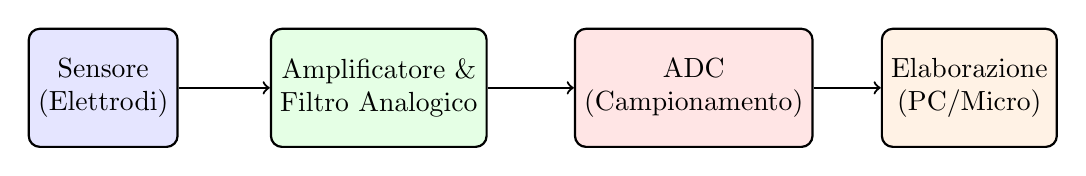
\begin{tikzpicture}[node distance=3cm, auto, thick]
        \node[draw, rectangle, rounded corners, fill=blue!10, minimum height=1.5cm, align=center] (sensor) {Sensore \\ (Elettrodi)};
        \node[draw, rectangle, rounded corners, fill=green!10, right of=sensor, node distance=3.5cm, minimum height=1.5cm, align=center] (amp) {Amplificatore \& \\ Filtro Analogico};
        \node[draw, rectangle, rounded corners, fill=red!10, right of=amp, node distance=4cm, minimum height=1.5cm, align=center] (adc) {ADC \\ (Campionamento)};
        \node[draw, rectangle, rounded corners, fill=orange!10, right of=adc, node distance=3.5cm, minimum height=1.5cm, align=center] (pc) {Elaborazione \\ (PC/Micro)};

        \draw[->] (sensor) -- (amp);
        \draw[->] (amp) -- (adc);
        \draw[->] (adc) -- (pc);
    \end{tikzpicture}
    \caption{Catena di acquisizione dei segnali fisologici bioelettrici.}
\end{figure}

In \verb|Esercizio_ECG.m| e \verb|Esercizio_GSR.m| sono state esplorate tecniche di lettura e plotting in ambienti come MATLAB, indispensabili per visualizzare e preparare i dati.

\section{Teoria del Campionamento e Quantizzazione}
Qualsiasi segnale fisiologico, essendo analogico e continuo, deve passare in un form factor digitale per poter essere elaborato dalla macchina.
\begin{itemize}
    \item \textbf{Campionamento}: Determinato dal teorema di Nyquist-Shannon.
    Fissata una frequenza massima $f_{max}$ del segnale di interesse, la frequenza di campionamento $f_s$ deve essere:
    \begin{equation}
        f_s > 2 f_{max}
    \end{equation}
    Rispettare questa condizione permette di evitare il fenomeno dell'\textbf{aliasing}. Nel caso di sottocampionamento o decimazione (riduzione intenzionale di $f_s$), si verifica un "ripiegamento" delle frequenze superiori a $f_s/2$ (frequenza di Nyquist) sulle frequenze inferiori. Questo effetto crea una distorsione nota come "effetto fisarmonica" nello spettro, rendendo impossibile la ricostruzione fedele del segnale originale.

    \vspace{0.5cm}
    \begin{figure}[h!]
        \centering
        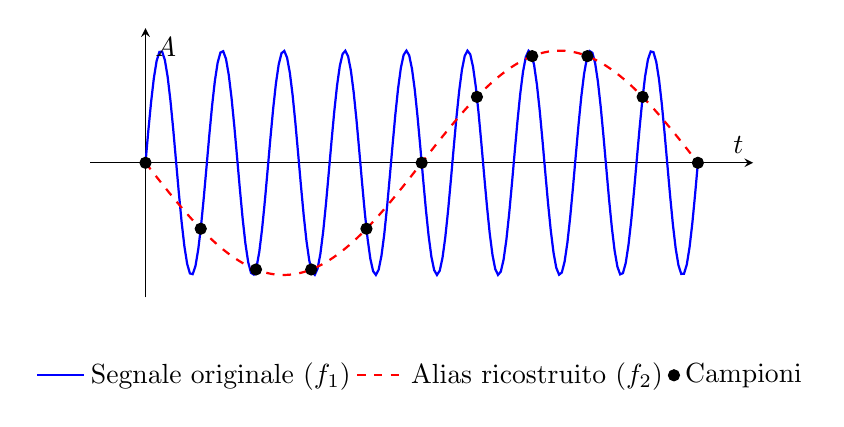
\begin{tikzpicture}
            \begin{axis}[
                width=10cm, height=5cm,
                domain=0:10, samples=200,
                axis lines=middle,
                xtick=\empty, ytick=\empty,
                xlabel=$t$, ylabel=$A$,
                enlargelimits=true,
                legend style={at={(0.5,-0.2)}, anchor=north, legend columns=-1, draw=none}
            ]
                \addplot[blue, thick] {sin(deg(2*pi*0.9*x))};
                \addlegendentry{Segnale originale ($f_1$)}
                \addplot[red, dashed, thick] {-sin(deg(2*pi*0.1*x))};
                \addlegendentry{Alias ricostruito ($f_2$)}
                \addplot[only marks, mark=*, samples=11] {sin(deg(2*pi*0.9*x))};
                \addlegendentry{Campioni}
            \end{axis}
        \end{tikzpicture}
        \caption{Fenomeno dell'aliasing: un segnale ad alta frequenza campionato troppo lentamente viene confuso con una bassa frequenza.}
    \end{figure}
    \vspace{0.5cm}

    \item \textbf{Quantizzazione}: Consiste nella mappatura di valori continui di ampiezza in un insieme finito di $L$ livelli discreti, definiti dal numero di bit $b$:
    \begin{equation}
        L = 2^b
    \end{equation}
    La distanza tra due livelli consecutivi, ovvero la \textbf{risoluzione (step d'intervallo)}, indicata con $\Delta$, è data formalmente da:
    \begin{equation}
        \Delta = \frac{x_{max} - x_{min}}{L}
    \end{equation}
    \textit{Nota: nella pratica e in alcuni esercizi, per mappare esattamente i valori limite tra 0 e $L-1$, è frequente calcolare lo step dividendo per $L-1$.}

    L'arrotondamento ai livelli produce un inevitabile \textbf{errore di quantizzazione}, assimilabile a un rumore additivo ed indipendente dal segnale in caso di risoluzione sufficiente. L'errore è confinato nell'intervallo $[-\Delta/2, \Delta/2]$.

    \vspace{0.5cm}
    \begin{figure}[h!]
        \centering
        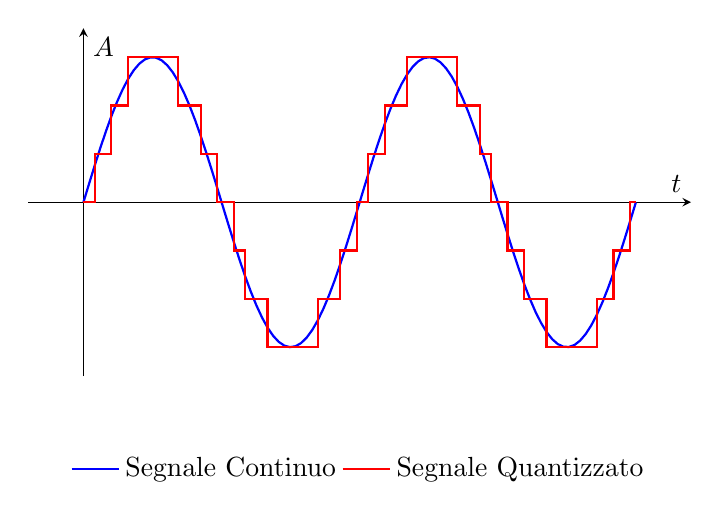
\begin{tikzpicture}
            \begin{axis}[
                width=10cm, height=6cm,
                domain=0:4*pi, samples=100,
                axis lines=middle,
                xtick=\empty, ytick=\empty,
                xlabel=$t$, ylabel=$A$,
                enlargelimits=true,
                legend style={at={(0.5,-0.2)}, anchor=north, legend columns=-1, draw=none}
            ]

            \addplot[blue, thick] {sin(deg(x))};
            \addlegendentry{Segnale Continuo}

            \addplot[red, thick, const plot] {round(sin(deg(x))*3)/3};
            \addlegendentry{Segnale Quantizzato}

            \end{axis}
        \end{tikzpicture}
        \caption{Quantizzazione: approssimazione del segnale continuo a livelli discreti (gradini).}
    \end{figure}
    \vspace{0.5cm}

    \item \textbf{Dithering}: È una tecnica usata nella quantizzazione che consiste nell'aggiunta volontaria di rumore bianco (con una particolare distribuzione probabilistica, es. densità di probabilità PDF triangolare o rettangolare) prima del quantizzatore per \emph{decorrelare} l'errore di quantizzazione dal segnale d'interesse, convertendo le distorsioni non-lineari e i toni spuri in un rumore di fondo uniforme, migliorando in media la fedeltà del segnale specialmente alle basse ampiezze.
\end{itemize}

\section{Energia, Potenza e Signal to Noise Ratio (SNR)}
L'acquisizione di segnali biologici è afflitta da instabilità e rumore, che può essere categorizzato in:
\begin{enumerate}
    \item \textbf{Rumore Termico (o bianco):} Inerente ai componenti elettronici, presente su tutto lo spettro con potenza pressoché costante (es. rumore gaussiano).
    \item \textbf{Artefatti da Movimento:} Causati dai micro-scivolamenti dell'elettrodo sulla pelle o movimenti muscolari. Si presenta spesso come variazioni di baseline a bassissima frequenza o picchi impulsivi (rumore spike).
    \item \textbf{Interferenza di Rete (Powerline noise):} Rumore a 50 Hz (in Europa) o 60 Hz causato dall'accoppiamento con l'impianto elettrico.
\end{enumerate}

Matematicamente, per caratterizzare un segnale valuto:
\begin{itemize}
    \item \textbf{Energia:}
    \\ Continuo: $\displaystyle E = \int_{-\infty}^{+\infty} |x(t)|^2 dt$
    \\ Discreto: $\displaystyle E = \sum_{n=-\infty}^{+\infty} |x[n]|^2$
    \vspace{0.2cm}
    \item \textbf{Potenza Media:}
    \\ Continuo: $\displaystyle P = \lim_{T \to \infty} \frac{1}{2T} \int_{-T}^{T} |x(t)|^2 dt$
    \\ Discreto: $\displaystyle P = \lim_{N \to \infty} \frac{1}{2N+1} \sum_{n=-N}^{N} |x[n]|^2$
\end{itemize}

Il \textbf{SNR (Signal-to-Noise Ratio)} è la metrica principale per definire la pulizia di un segnale rispetto ai disturbi acquisiti dai sensori o creati dai circuiti:
\begin{equation}
    SNR_{dB} = 10 \log_{10} \left( \frac{P_{seg}}{P_{rum}} \right)
\end{equation}
Maggiore è l'SNR, migliore è la qualità dell'informazione.
Nel caso specifico del rumore introdotto dalla sola quantizzazione, possiamo calcolare empiricamente il Signal-to-Quantization-Noise Ratio (SQNR) in decibel in base al numero di bit $b$:
\begin{equation}
    SQNR \approx 6.02 \cdot b + 1.76 \text{ [dB]}
\end{equation}

\section{Approfondimento sui Segnali Fisiologici (ECG e EDA)}
\subsection{Segnale ECG (Elettrocardiogramma)}
L'ECG evidenzia il funzionamento cardiaco.
È caratterizzato, nel singolo battito, dal \textbf{complesso QRS} (depolarizzazione dei ventricoli), che presenta il picco R primario.
Lo studio si basa sull'\textbf{HRV (Heart Rate Variability)}, che è la variazione nel tempo tra un battito e il successivo.
Gli intervalli R-R sono usati per estrarre metriche fondamentali:
\begin{itemize}
    \item \textbf{SDNN:} Deviazione standard degli intervalli N-N (R-R normali), denota variabilità a lungo termine.
    \item \textbf{RMSSD:} Root mean square successive difference, che riflette l'influenza parasimpatica immediata.
\end{itemize}
Spesso il segnale ECG presenta una deriva della linea di base (baseline wander) attribuibile alla respirazione e ai movimenti.
Viene facilmente compensata con tecniche di regressione polinomiale o operando una funzione \texttt{detrend}.

\subsection{Segnale EDA/GSR (Electrodermal Activity)}
I segnali galvanici (GSR) variano con la sudorazione del palmo o delle dita.
Questo segnale è composto dalla somma di due parti distinte da separare algoritmicamente:
\begin{itemize}
    \item \textbf{Componente Tonica (SCL - Skin Conductance Level):} Molto lenta, misurabile in periodi prolungati; indica uno stato generale (es.
    stress a lungo termine, allerta prolungata).
    Subisce fenomeni di drift nel tempo.
    Si estrae per esempio con un filtro passa-basso con taglio a $\sim$ 0.05 Hz.
    \item \textbf{Componente Fasica (SCR - Skin Conductance Response):} Estremamente veloce, sovrapposta alla tonica; rappresenta le reazioni istantanee a stimoli emotivi specifici (es.
    paura, sorpresa).
    Presenta dei \emph{picchi} tipici.
    Isolata rimuovendo la tonica, si usa solitamente un passa-basso a $\sim$ 1-2 Hz.
\end{itemize}

\section{Filtraggio e Tecniche di Denoising}
Per pulire i segnali vengono adoperati vari filtri di elaborazione del segnale digitale:
\begin{description}
    \item[Filtri Passa-Basso, Passa-Alto e Passa-Banda:] Rimuovono componenti di frequenza specifiche.
    Tra i filtri standard vi è il \textbf{Filtro Butterworth}, che è massimamente piatto in banda passante.
    La pendenza (roll-off) del filtro è direttamente legata all'\emph{ordine} del filtro.
    Attenzione: aumentare troppo l'ordine porta a instabilità e fenomeni di \emph{ringing} (oscillazioni spurie o sovraelongazioni pre e post-filtro).
    \item[Frequenza Lineari vs Non-Lineari (Media vs Mediano):] \mbox{} \\
    \begin{itemize}
        \item Il \textbf{Filtro della Media (Moving Average)} è un filtro lineare. L'equazione per una finestra di dimensione $W$ (dispari, con $k=(W-1)/2$) è:
        \begin{equation}
            y[n] = \frac{1}{W} \sum_{i=-k}^{k} x[n-i]
        \end{equation}
        È ottimo per attenuare rumore bianco (gaussiano).
        Tuttavia, in presenza di un rumore impulsivo (outlier), la media ne risente e finisce per "spalmare" l'errore sui campioni vicini, addolcendo eccessivamente i fronti di salita (bordi netti).

        \item Il \textbf{Filtro Mediano} è un operatore di rango \textbf{non lineare}. L'equazione è:
        \begin{equation}
            y[n] = \text{mediano}( \{ x[n-k], \dots, x[n], \dots, x[n+k] \} )
        \end{equation}
        Eccellente e robusto per scartare rumori impulsivi (spike o salt \& pepper): un singolo valore outlier viene completamente ignorato dal calcolo del mediano; in più, esso riesce a preservare in modo intatto i fronti di salita rapidi del segnale, risultando essenziale in morfologie a gradino o picchi importanti.
    \end{itemize}
\end{description}

\vspace{0.5cm}
\begin{table}[h!]
    \centering
    \begin{tabular}{|p{4.5cm}|p{5cm}|p{5cm}|}
        \hline
        \textbf{Caratteristica} & \textbf{Filtro Media (Moving Avg)} & \textbf{Filtro Mediano} \\
        \hline
        \textbf{Tipo} & Lineare & Non Lineare \\
        \hline
        \textbf{Rumore Gaussiano} & Attenua bene & Distorce leggermente \\
        \hline
        \textbf{Rumore Impulsivo (Spike)} & Spalma l'errore (inefficace) & Elimina lo spike (ottimo) \\
        \hline
        \textbf{Bordi netti / Gradini} & Addolcisce (sfoca) & Preserva intatti \\
        \hline
    \end{tabular}
    \caption{Tabella comparativa: Filtro Media vs Filtro Mediano.}
\end{table}
\vspace{0.5cm}
